\documentclass{article}

\usepackage[papersize={34.2cm,23.18cm},left=0cm,right=0cm,top=0cm,bottom=0cm]{geometry}
\usepackage{tikz}
\usetikzlibrary{backgrounds,mindmap}

\definecolor{f1}{HTML}{7FA0A0}
\definecolor{f2}{HTML}{1133FF}
\definecolor{f3}{HTML}{36648B}
\definecolor{f7}{HTML}{5692B4}
\definecolor{f5}{HTML}{78BCEE}
\definecolor{f6}{HTML}{00FFFF}
\definecolor{f9}{HTML}{00DD99}
\definecolor{f8}{HTML}{FFFFA6}
\definecolor{f4}{HTML}{00CC66}
\definecolor{f10}{HTML}{00BB22}
\definecolor{darkgreen}{HTML}{006600}
\definecolor{scipyellow}{HTML}{FFFFE6}

\pagestyle{empty}

\begin{document}
\centering
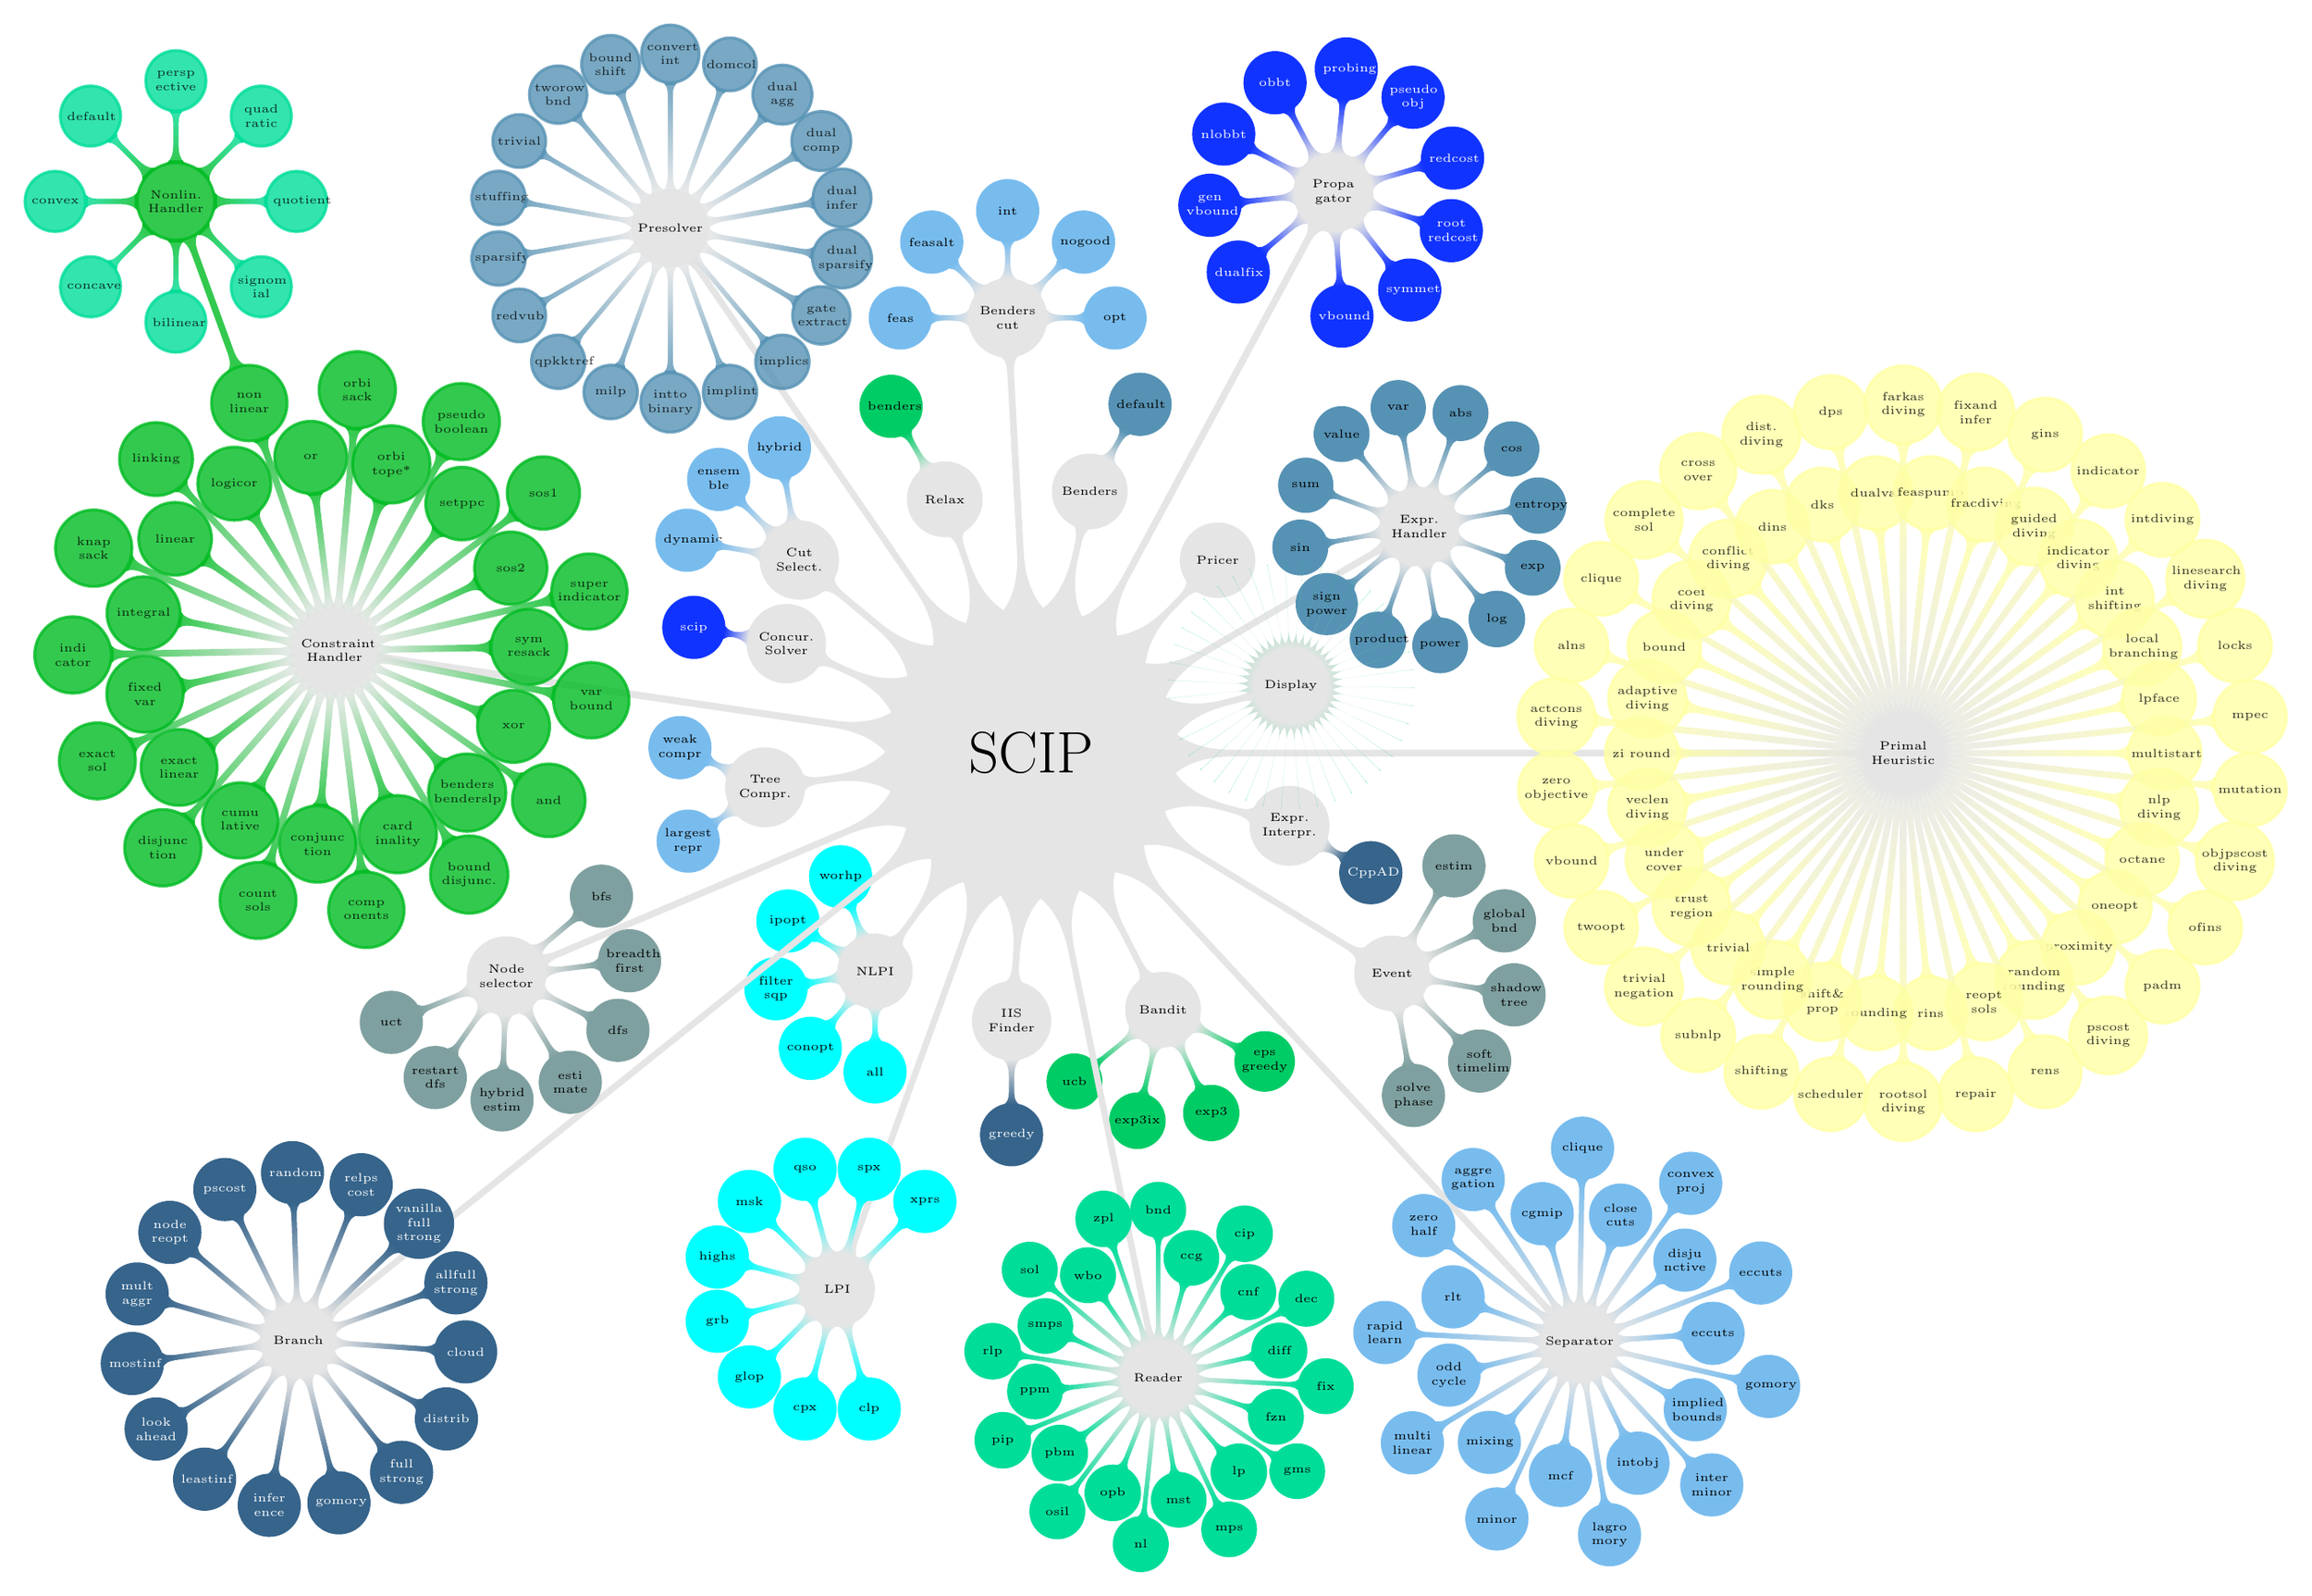
\begin{tikzpicture}[mindmap,concept color=gray!20]
  %\tikzstyle{root concept} = [concept, text width=1cm, minimum size=1cm];
  \tikzstyle{level 1 concept} = [level 3 concept,level distance=3.7cm,sibling angle=18, minimum size=.7cm];
  \tikzstyle{level 2 concept} = [level 4 concept];%sibling angle=18, minimum size=1cm, text width=1cm];
  \tikzstyle{scipconcept} = [concept, level distance=4cm, sibling angle=15.7, minimum size=.4cm];
  \tikzstyle{branchconcept} = [level 2 concept, level distance=2.5cm, sibling angle=24, concept color=f3,text=white];
  \tikzstyle{conshdlrconcept} = [level 1 concept,sibling angle=12,concept color=f10,minimum size=.6cm,opacity=0.8];
  \tikzstyle{conshdlrconceptodd} = [conshdlrconcept, level distance=3.9cm];
  \tikzstyle{conshdlrconcepteven} = [conshdlrconcept, level distance=2.9cm];
  \tikzstyle{lpiconcept} = [level 2 concept,concept color=f6];
  \tikzstyle{dialogconcept} = [level 2 concept,concept color=f4];
  \tikzstyle{displayconcept} = [level 2 concept,sibling angle=8.5,concept color=f4];
  \tikzstyle{nodeselectionconcept} = [level 2 concept,sibling angle=33,concept color=f1];
  \tikzstyle{presolverconcept} = [level 2 concept,sibling angle=20,level distance=2.6cm,concept color=f7, minimum size=.4cm,opacity=0.8];
  \tikzstyle{heurconcepteven} = [level 1 concept, sibling angle=6, level distance=5.2cm, concept color=f8, minimum size=.4cm, opacity=0.8];
  \tikzstyle{heurconceptodd} = [heurconcepteven, level distance=3.9cm];
  \tikzstyle{readerconceptodd} = [level 2 concept,sibling angle=15.5,concept color=f9, minimum size=.4cm];
  \tikzstyle{readerconcepteven} = [readerconceptodd, level distance=2.5cm];
  \tikzstyle{sepaconcept} = [level 2 concept,sibling angle=17, concept color=f5];
  \tikzstyle{sepaconceptodd} = [sepaconcept,level distance=2cm];
  \tikzstyle{sepaconcepteven} = [sepaconcept,level distance=2.9cm];
  \tikzstyle{propconcept} = [level 2 concept,sibling angle=34,concept color=f2,text = white];
  \tikzstyle{eventconcept} = [level 2 concept,sibling angle=35,concept color=f1];
  \tikzstyle{nlpiconcept} = [level 2 concept, level distance=1.5cm,sibling angle=40,concept color=f6];
  \tikzstyle{exprintconcept} = [level 2 concept, level distance=1.4cm,concept color=f3,text=white];
  \tikzstyle{relaxconcept} = [level 2 concept, level distance=1.6cm,concept color=f4];
  \tikzstyle{conflictconcept} = [level 2 concept, level distance=1.7cm,sibling angle=40,concept color=f4];
  \tikzstyle{nlhdlrconcept} = [level 4 concept, sibling angle=45, level distance=1.8cm, concept color=f9];
  \tikzstyle{comprconcept} = [level 2 concept, level distance=1.4cm, sibling angle=60,concept color=f5];
  \tikzstyle{bendersconcept} = [level 2 concept, level distance=1.5cm, concept color=f7];
  \tikzstyle{benderscutconcept} = [level 2 concept, level distance=1.6cm, sibling angle=45, concept color=f5];
  \tikzstyle{concsolverconcept} = [level 2 concept, level distance=1.4cm, concept color=f2,text=white];
  \tikzstyle{cutselconcept} = [level 2 concept, level distance=1.7cm, sibling angle=35, concept color=f5];
  \tikzstyle{iisfinderconcept} = [level 2 concept, level distance=1.7cm, concept color=f3,text=white];
  \tikzstyle{exprconcept} = [level 2 concept, level distance=1.8cm, concept color=f7,minimum size=.4cm];
  \tikzstyle{banditconcept} = [level 2 concept, level distance=1.7cm, sibling angle=38,concept color=f4,minimum size=.4cm];
  % this style is used to mark plugins that are not included by GCG (gcgplugins.c)

  \node [concept] {\Huge SCIP}
  [clockwise from=0]
  child[scipconcept,level distance=13cm] { node[concept, minimum size=1cm] (Heuristic) {Primal\\Heuristic}
    [clockwise from=174]
    child[heurconcepteven] { node[concept] (actconsdiving) {actcons\\diving}}
    child[heurconceptodd] { node[concept] (adaptivediving) {adaptive\\diving}}
    child[heurconcepteven] { node[concept] (alns) {alns}}
    child[heurconceptodd] { node[concept] (bound) {bound}}
    child[heurconcepteven]  { node[concept] (clique) {clique}}
    child[heurconceptodd]  { node[concept] (coefdiving) {coef\\diving}}
    child[heurconcepteven] { node[concept] (completesol) {complete\\sol}}
    child[heurconceptodd] { node[concept] (conflictdiving) {conflict\\diving}}
    child[heurconcepteven] { node[concept] (crossover) {cross\\over}}
    child[heurconceptodd]  { node[concept] (dins) {dins}}
    child[heurconcepteven]  { node[concept] (distribdiving) {dist.\\diving}}
    child[heurconceptodd]  { node[concept] (dks) {dks}}
    child[heurconcepteven]  { node[concept] (dps) {dps}}
    child[heurconceptodd] { node[concept] (dualval) {dualval}}
    child[heurconcepteven]  { node[concept] (farkasdiving) {farkas\\diving}}
    child[heurconceptodd]  { node[concept] (feaspump) {feaspump}}
    child[heurconcepteven] { node[concept] (fixandinfer) {fixand\\infer}}
    child[heurconceptodd]  { node[concept] (fracdiving) {fracdiving}}
    child[heurconcepteven]  { node[concept] (gins) {gins}}
    child[heurconceptodd] { node[concept] (guideddiving) {guided\\diving}}
    child[heurconcepteven]   { node[concept] (indicator) {indicator}}
    child[heurconceptodd]   { node[concept] (indicatordiving) {indicator\\diving}}
    child[heurconcepteven]  { node[concept] (intdiving) {intdiving}}
    child[heurconceptodd]   { node[concept] (intshifting) {int\\shifting}}
    child[heurconcepteven]  { node[concept] (linesearchdiving) {linesearch\\diving}}
    child[heurconceptodd]   { node[concept] (localbranching) {local\\branching}}
    child[heurconcepteven]  { node[concept] (locks) {locks}}
    child[heurconceptodd]  { node[concept] (lpface) {lpface}}
    child[heurconcepteven]  { node[concept] (mpec) {mpec}}
    child[heurconceptodd]  { node[concept] (multistart) {multistart}}
    child[heurconcepteven]  { node[concept] (mutation) {mutation}}
    child[heurconceptodd]  { node[concept] (nlpdiving) {nlp\\diving}}
    child[heurconcepteven]  { node[concept] (objpscostdiving) {objpscost\\diving}}
    child[heurconceptodd]   { node[concept] (octane) {octane}}
    child[heurconcepteven]  { node[concept] (ofins) {ofins}}
    child[heurconceptodd] { node[concept] (oneopt) {oneopt}}
    child[heurconcepteven]   { node[concept] (padm) {padm}}
    child[heurconceptodd]   { node[concept] (proximity) {proximity}}
    child[heurconcepteven]  { node[concept] (pscostdiving) {pscost\\diving}}
    child[heurconceptodd]  { node[concept] (randround) {random\\rounding}}
    child[heurconcepteven]   { node[concept] (rens) {rens}}
    child[heurconceptodd]  { node[concept] (reoptsols) {reopt\\sols}}
    child[heurconcepteven]   { node[concept] (repair) {repair}}
    child[heurconceptodd]   { node[concept] (rins) {rins}}
    child[heurconcepteven]  { node[concept] (rootsoldiving) {rootsol\\diving}}
    child[heurconceptodd]   { node[concept] (rounding) {rounding}}
    child[heurconcepteven]  { node[concept] (scheduler) {scheduler}}
    child[heurconceptodd]  { node[concept] (shiftandpropagate) {shift\&\\prop}}
    child[heurconcepteven]  { node[concept] (shifting) {shifting}}
    child[heurconceptodd]   { node[concept] (simplerounding) {simple\\rounding}}
    child[heurconcepteven]   { node[concept] (subnlp) {subnlp}}
    %child[heurconcepteven]   { node[concept] (sync) {sync}}
    child[heurconceptodd]  { node[concept] (trivial) {trivial}}
    child[heurconcepteven]  { node[concept] (trivialnegation) {trivial\\negation}}
    child[heurconceptodd]  { node[concept] (trustregion) {trust\\region}}
    %child[heurconceptodd]    { node[concept] (trysol) {trysol}}
    child[heurconcepteven]  { node[concept] (twoopt) {twoopt}}
    child[heurconceptodd]    { node[concept] (undercover) {under\\cover}}
    child[heurconcepteven] { node[concept] (vbounds) {vbound}}
    child[heurconceptodd]   { node[concept] (veclendiving) {veclen\\diving}}
    child[heurconcepteven]  { node[concept] (zeroobj) {zero\\objective}}
    child[heurconceptodd] { node[concept] (ziround) {zi round}}
  }
  child[scipconcept] { node[concept] (Exprint) {Expr. Interpr.}
     [clockwise from=-30]
     child[exprintconcept] { node[concept] (cppad) {CppAD}}
   }
  child[scipconcept,level distance=6.3cm] { node[concept] (Event) {Event}
     [clockwise from=60]
     child[eventconcept] { node[concept] (estim) {estim}}
     child[eventconcept] { node[concept] (globalbnd) {global\\bnd}}
     child[eventconcept] { node[concept] (shadowtree) {shadow\\tree}}
     child[eventconcept] { node[concept] (softtime) {soft\\timelim}}
     child[eventconcept] { node[concept] (solvingphase) {solve\\phase}}
  }
  child[scipconcept,level distance=12cm] { node[concept] (Separator) {Separator}
    [clockwise from=123]
    child[sepaconcepteven] { node[concept] (aggr) {aggre\\gation}}
    child[sepaconceptodd] { node[concept] (cgmip) {cgmip}}
    child[sepaconcepteven] { node[concept] (clique) {clique}}
    child[sepaconceptodd] { node[concept] (closecuts) {close\\cuts}}
    child[sepaconcepteven] { node[concept] (convexproj) {convex\\proj}}
    child[sepaconceptodd] { node[concept] (disjunctive) {disju\\nctive}}
    child[sepaconcepteven] { node[concept] (eccuts) {eccuts}}
    child[sepaconceptodd] { node[concept] (gauge) {eccuts}}
    child[sepaconcepteven] { node[concept] (gomory) {gomory}}
    child[sepaconceptodd] { node[concept] (impliedbounds) {implied\\bounds}}
    child[sepaconcepteven] { node[concept] (interminor) {inter\\minor}}
    child[sepaconceptodd] { node[concept] (intobj) {intobj}}
    child[sepaconcepteven] { node[concept] (lagromory) {lagro\\mory}}
    child[sepaconceptodd] { node[concept] (mcf) {mcf}}
    child[sepaconcepteven] { node[concept] (minor) {minor}}
    child[sepaconceptodd] { node[concept] (mixing) {mixing}}
    child[sepaconcepteven] { node[concept] (multilinear) {multi\\linear}}
    child[sepaconceptodd] { node[concept] (oddcycle) {odd\\cycle}}
    child[sepaconcepteven] { node[concept] (rapidlearning) {rapid\\learn}}
    child[sepaconceptodd] { node[concept] (rlt) {rlt}}
    child[sepaconcepteven] { node[concept] (zerohalf) {zero\\half}}
  }
  child[scipconcept,level distance=4.3cm] { node[concept] (bandit) {Bandit}
    [clockwise from=-27]
    child[banditconcept] { node[concept] (epsgreedy) {eps\\greedy}}
    child[banditconcept] { node[concept] (exp3) {exp3}}
    child[banditconcept] { node[concept] (exp3ix) {exp3ix}}
    child[banditconcept] { node[concept] (ucb) {ucb}}
  }
  child[scipconcept,level distance=9.5cm] { node[concept] (Reader) {Reader}
    [clockwise from=90]
    child[readerconcepteven] { node[concept] (bnd) {bnd}}
    child[readerconceptodd] { node[concept] (ccg) {ccg}}
    child[readerconcepteven] { node[concept] (cip) {cip}}
    child[readerconceptodd] { node[concept] (cnf) {cnf}}
    %child[readerconceptodd] { node[concept] (cor) {cor}}
    child[readerconcepteven] { node[concept] (dec) {dec}}
    child[readerconceptodd] { node[concept] (diff) {diff}}
    child[readerconcepteven] { node[concept] (fix) {fix}}
    child[readerconceptodd] { node[concept] (fzn) {fzn}}
    child[readerconcepteven] { node[concept] (gms) {gms}}
    child[readerconceptodd] { node[concept] (lp) {lp}}
    child[readerconcepteven] { node[concept] (mps) {mps}}
    child[readerconceptodd] { node[concept] (mst) {mst}}
    child[readerconcepteven] { node[concept] (nl) {nl}}
    child[readerconceptodd] { node[concept] (opb) {opb}}
    child[readerconcepteven] { node[concept] (osil) {osil}}
    child[readerconceptodd] { node[concept] (pbm) {pbm}}
    child[readerconcepteven] { node[concept] (pip) {pip}}
    child[readerconceptodd] { node[concept] (ppm) {ppm}}
    child[readerconcepteven] { node[concept] (rlp) {rlp}}
    child[readerconceptodd] { node[concept] (smps) {smps}}
    child[readerconcepteven] { node[concept] (sol) {sol}}
    %child[readerconceptodd] { node[concept] (sto) {sto}}
    %child[readerconceptodd] { node[concept] (tim) {tim}}
    child[readerconceptodd] { node[concept] (wbo) {wbo}}
    child[readerconcepteven] { node[concept] (zpl) {zpl}}
  }
  child[scipconcept] { node[concept] (iisfinder) {IIS\\Finder}
    [clockwise from=-90]
    child[iisfinderconcept] { node[concept] (greedy) {greedy}}
  }
  child[scipconcept,level distance=8.5cm] { node[concept] (LPI) {LPI}
    [clockwise from=-75]
    child[lpiconcept] { node[concept] (clp) {clp}}
    child[lpiconcept] { node[concept] (cpx) {cpx}}
    child[lpiconcept] { node[concept] (glop) {glop}}
    child[lpiconcept] { node[concept] (grb) {grb}}
    child[lpiconcept] { node[concept] (highs) {highs}}
    child[lpiconcept] { node[concept] (msk) {msk}}
    child[lpiconcept] { node[concept] (qso) {qso}}
    child[lpiconcept] { node[concept] (spx) {spx}}
    child[lpiconcept] { node[concept] (xprs) {xprs}}
  }
  child[scipconcept] { node[concept] (NLPI) {NLPI}
    [clockwise from=-90]
    child[nlpiconcept] { node[concept] (all) {all}}
    child[nlpiconcept] { node[concept] (conopt) {conopt}}
    child[nlpiconcept] { node[concept] (filtersqp) {filter\\sqp}}
    child[nlpiconcept] { node[concept] (ipopt) {ipopt}}
    child[nlpiconcept] { node[concept] (worhp) {worhp}}
  }
  child[scipconcept,level distance=14cm] { node[concept] (Branch) {Branch}
    [clockwise from=20]
    child[branchconcept] { node[concept] (allfullstring) {allfull\\strong}}
    child[branchconcept] { node[concept] (cloud) {cloud}}
    child[branchconcept] { node[concept] (distribution) {distrib}}
    child[branchconcept] { node[concept] (fullstrong) {full\\strong}}
    child[branchconcept] { node[concept] (gomory) {gomory}}
    child[branchconcept] { node[concept] (inference) {infer\\ence}}
    child[branchconcept] { node[concept] (leastinf) {leastinf}}
    child[branchconcept] { node[concept] (lookahead) {look\\ahead}}
    child[branchconcept] { node[concept] (mostinf) {mostinf}}
    child[branchconcept] { node[concept] (multaggr) {mult\\aggr}}
    child[branchconcept] { node[concept] (nodereopt) {node\\reopt}}
    child[branchconcept] { node[concept] (pscost) {pscost}}
    child[branchconcept] { node[concept] (random) {random}}
    child[branchconcept] { node[concept] (relpscost) {relps\\cost}}
    child[branchconcept] { node[concept] (vanillastrong) {vanilla\\full\\strong}}
  }
  child[scipconcept,level distance=8.5cm] { node[concept] (Nodeselector) {Node\\selector}
    [clockwise from=40]
    child[nodeselectionconcept] { node[concept] (bfs) {bfs}}
    child[nodeselectionconcept] { node[concept] (breadth) {breadth\\first}}
    child[nodeselectionconcept] { node[concept] (dfs) {dfs}}
    child[nodeselectionconcept] { node[concept] (estimate) {esti\\mate}}
    child[nodeselectionconcept] { node[concept] (hybridestim) {hybrid\\estim}}
    child[nodeselectionconcept] { node[concept] (restartdfs) {restart\\dfs}}
    child[nodeselectionconcept] { node[concept] (uct) {uct}}
  }
  child[scipconcept] { node[concept] (compr) {Tree\\Compr.}
    [clockwise from=-145]
    child[comprconcept] { node[concept] (largestrepr) {largest\\repr}}
    child[comprconcept] { node[concept] (weakcompr) {weak\\compr}}
  }
  child[scipconcept,level distance=10.5cm,minimum size=1.2cm] { node[concept] (ConsHdlr) {Constraint\\Handler}
    [clockwise from=-35]
    child[conshdlrconceptodd] { node[concept] (and) {and}}
    child[conshdlrconcepteven] { node[concept] (benders) {benders\\benderslp}}
    child[conshdlrconceptodd] { node[concept] (bounddisjunction) {bound\\disjunc.}}
    child[conshdlrconcepteven] { node[concept] (cardinality) {card\\inality}}
    child[conshdlrconceptodd] { node[concept] (components) {comp\\onents}}
    child[conshdlrconcepteven] { node[concept] (conjunction) {conjunc\\tion}}
    child[conshdlrconceptodd] { node[concept] (countsols) {count\\sols}}
    child[conshdlrconcepteven] { node[concept] (cumulative) {cumu\\lative}}
    child[conshdlrconceptodd] { node[concept] (disjunction) {disjunc\\tion}}
    child[conshdlrconcepteven] { node[concept] (exactlinear) {exact\\linear}}
    child[conshdlrconceptodd] { node[concept] (exactsol) {exact\\sol}}
    child[conshdlrconcepteven] { node[concept] (fixedvar) {fixed\\var}}
    child[conshdlrconceptodd] { node[concept] (indicator) {indi\\cator}}
    child[conshdlrconcepteven] { node[concept] (integral) {integral}}
    child[conshdlrconceptodd] { node[concept] (knapsack) {knap\\sack}}
    child[conshdlrconcepteven] { node[concept] (linear) {linear}}
    child[conshdlrconceptodd] { node[concept] (linking) {linking}}
    child[conshdlrconcepteven] { node[concept] (logicor) {logicor}}
    child[conshdlrconceptodd] { node[concept] (nonlinear) {non\\linear}
      child[level distance=3.2cm,grow=110] { node[concept] (nlhdlr) {Nonlin.\\Handler}
      [clockwise from=-90]
        child[nlhdlrconcept] { node[concept] (bilinear) {bilinear}}
        child[nlhdlrconcept] { node[concept] (concave) {concave}}
        child[nlhdlrconcept] { node[concept] (convex) {convex}}
        child[nlhdlrconcept] { node[concept] (default) {default}}
        child[nlhdlrconcept] { node[concept] (perspective) {persp\\ective}}
        child[nlhdlrconcept] { node[concept] (quadratic) {quad\\ratic}}
        child[nlhdlrconcept] { node[concept] (quotient) {quotient}}
        child[nlhdlrconcept] { node[concept] (signomial) {signom\\ial}}
      }
    }
    child[conshdlrconcepteven] { node[concept] (or) {or}}
    child[conshdlrconceptodd] { node[concept] (orbisack) {orbi\\sack}}
    child[conshdlrconcepteven] { node[concept] (orbitope) {orbi\\tope*}}
    child[conshdlrconceptodd] { node[concept] (pseudoboolean) {pseudo\\boolean}}
    child[conshdlrconcepteven] { node[concept] (setppc) {setppc}}
    child[conshdlrconceptodd] { node[concept] (sos1) {sos1}}
    child[conshdlrconcepteven] { node[concept] (sos2) {sos2}}
    child[conshdlrconceptodd] { node[concept] (superindicator) {super\\indicator}}
    child[conshdlrconcepteven] { node[concept] (symresack) {sym\\resack}}
    child[conshdlrconceptodd] { node[concept] (varbound) {var\\bound}}
    child[conshdlrconcepteven] { node[concept] (xor) {xor}}
  }
  child[scipconcept] { node[concept] (concsolver) {Concur.\\Solver}
    [clockwise from=170]
    child[concsolverconcept] { node[concept] (scip) {scip}}
  }
  child[scipconcept,level distance=4.5cm] { node[concept] (cutsel) {Cut\\Select.}
    [clockwise from=170]
    child[cutselconcept] { node[concept] (dynamic) {dynamic}}
    child[cutselconcept] { node[concept] (ensemble) {ensem\\ble}}
    child[cutselconcept] { node[concept] (hybrid) {hybrid}}
  }
%   child { node[concept] (Display) {Display}
%     [clockwise from=-155]
%     child[displayconcept] { node[concept] (default) {default}}
%   }
  child[scipconcept,level distance=9.5cm] { node[concept] (Presolver) {Presolver}
    [clockwise from=110]
    child[presolverconcept] { node[concept] (boundshift) {bound\\shift}}
    child[presolverconcept] { node[concept] (convertinttobinary) {convert\\int}}
    child[presolverconcept] { node[concept] (domcol) {domcol}}
    child[presolverconcept] { node[concept] (dualagg) {dual\\agg}}
    child[presolverconcept] { node[concept] (dualcomp) {dual\\comp}}
    child[presolverconcept] { node[concept] (dualinfer) {dual\\infer}}
    child[presolverconcept] { node[concept] (dualsparsify) {dual\\sparsify}}
    child[presolverconcept] { node[concept] (gateextract) {gate\\extract}}
    child[presolverconcept] { node[concept] (implics) {implics}}
    child[presolverconcept] { node[concept] (implint) {implint}}
    child[presolverconcept] { node[concept] (inttobinary) {intto\\binary}}
    child[presolverconcept] { node[concept] (milp) {milp}}
    child[presolverconcept] { node[concept] (qpkktref) {qpkktref}}
    child[presolverconcept] { node[concept] (redvub) {redvub}}
    child[presolverconcept] { node[concept] (sparsify) {sparsify}}
    child[presolverconcept] { node[concept] (stuffing) {stuffing}}
    child[presolverconcept] { node[concept] (trivial) {trivial}}
    child[presolverconcept] { node[concept] (tworowbnd) {tworow\\bnd}}
  }
  child[scipconcept] { node[concept] (Relaxer) {Relax}
    [clockwise from=120]
    child[relaxconcept] { node[concept] (benders) {benders}}
  }
  child[scipconcept,level distance=6.5cm] { node[concept] (benderscut) {Benders\\cut}
    [clockwise from=180]
    child[benderscutconcept] { node[concept] (feas) {feas}}
    child[benderscutconcept] { node[concept] (feasalt) {feasalt}}
    child[benderscutconcept] { node[concept] (int) {int}}
    child[benderscutconcept] { node[concept] (nogood) {nogood}}
    child[benderscutconcept] { node[concept] (opt) {opt}}
  }
  child[scipconcept] { node[concept] (benders) {Benders}
    [clockwise from=60]
    child[bendersconcept] { node[concept] (default) {default}}
  }
  child[scipconcept,level distance=9.5cm] { node[concept] (Propagator) {Propa\\gator}
    [clockwise from=220]
    child[propconcept] { node[concept] (dualfix) {dualfix}}
    child[propconcept] { node[concept] (genvbounds) {gen\\vbound}}
    child[propconcept] { node[concept] (nlobbt) {nlobbt}}
    child[propconcept] { node[concept] (obbt) {obbt}}
    child[propconcept] { node[concept] (probing) {probing}}
    child[propconcept] { node[concept] (pseudoobj) {pseudo\\obj}}
    child[propconcept] { node[concept] (redcost) {redcost}}
    child[propconcept] { node[concept] (rootredcost) {root\\redcost}}
    child[propconcept] { node[concept] (symmetry) {symmetry}}
    child[propconcept] { node[concept] (vbounds) {vbound}}
  }
  % conflict handling is not implemented in plugins...
  %child[scipconcept,level distance=11.5cm] { node[concept] (Conflict) {Conflict}
  %  [clockwise from=90]
  %  child[conflictconcept] { node[concept] (dualproof) {dualpr.\\analysis}}
  %  child[conflictconcept] { node[concept] (general) {general}}
  %  child[conflictconcept] { node[concept] (graphanalysis) {graph\\analysis}}
  %  child[conflictconcept] { node[concept] (resolution) {reso\\lution}}
  %}
  child[scipconcept] { node[concept] (Pricer) {Pricer}}
  child[scipconcept,level distance=6.7cm] { node[concept] (exprhdlr) {Expr.\\Handler}
    [clockwise from=70]
    child[exprconcept] { node[concept] (abs) {abs}}
    child[exprconcept] { node[concept] (cos) {cos}}
    %erf
    child[exprconcept] { node[concept] (entropy) {entropy}}
    child[exprconcept] { node[concept] (exp) {exp}}
    child[exprconcept] { node[concept] (log) {log}}
    child[exprconcept] { node[concept] (pow) {power}}
    child[exprconcept] { node[concept] (product) {product}}
    child[exprconcept] { node[concept] (signpow) {sign\\power}}
    child[exprconcept] { node[concept] (sin) {sin}}
    child[exprconcept] { node[concept] (sum) {sum}}
    child[exprconcept] { node[concept] (value) {value}}
    child[exprconcept] { node[concept] (var) {var}}
    %varidx
  }
  child[scipconcept] { node[concept] (Display) {Display}
    [clockwise from=-174]
    child[displayconcept] { }
    child[displayconcept] { }
    child[displayconcept] { }
    child[displayconcept] { }
    child[displayconcept] { }
    child[displayconcept] { }
    child[displayconcept] { }
    child[displayconcept] { }
    child[displayconcept] { }
    child[displayconcept] { }
    child[displayconcept] { }
    child[displayconcept] { }
    child[displayconcept] { }
    child[displayconcept] { }
    child[displayconcept] { }
    child[displayconcept] { }
    child[displayconcept] { }
    child[displayconcept] { }
    child[displayconcept] { }
    child[displayconcept] { }
    child[displayconcept] { }
    child[displayconcept] { }
    child[displayconcept] { }
    child[displayconcept] { }
    child[displayconcept] { }
    child[displayconcept] { }
    child[displayconcept] { }
    child[displayconcept] { }
    child[displayconcept] { }
    child[displayconcept] { }
    child[displayconcept] { }
    child[displayconcept] { }
    child[displayconcept] { }
    child[displayconcept] { }
    child[displayconcept] { }
    child[displayconcept] { }
    child[displayconcept] { }
    child[displayconcept] { }
    child[displayconcept] { }
    child[displayconcept] { }
    child[displayconcept] { }
  }
  %child { node[concept] (Dialog) {Dialog}
  % [clockwise from=70]
  %  child[dialogconcept] { node[concept] (default) {default}}
  %}
  %message
  %table
;
\end{tikzpicture}

\end{document}
